\documentclass[twocolumn]{article}
\usepackage{mathpazo}
%david added
\usepackage{amsmath}
\usepackage{geometry}                % See geometry.pdf to learn the layout options. There are lots.
\geometry{letterpaper}                   % ... or a4paper or a5paper or ... 
%\geometry{landscape}                % Activate for for rotated page geometry
%\usepackage[parfill]{parskip}    % Activate to begin paragraphs with an empty line rather than an indent
\usepackage{graphicx}
\usepackage{epstopdf}

%end david added
\usepackage{microtype}
\usepackage{amsmath}
\usepackage[citecolor=Fuchsia,urlcolor=blue,linkcolor=Cerulean]{hyperref}
\usepackage{graphicx}
\usepackage{float}
\graphicspath{ {images/} {images/dd/} {images/greedy/} {images/qlearning/} }

\setlength\textwidth{7in} 
\setlength\textheight{9.5in} 
\setlength\oddsidemargin{-0.25in} 
\setlength\topmargin{-0.25in} 
\setlength\headheight{0in} 
\setlength\headsep{0in} 
\setlength\columnsep{18pt}
\sloppy 
 
\begin{document}

\title{
\vspace{-0.5in}\rule{\textwidth}{2pt}
\begin{tabular}{ll}\begin{minipage}{4.75in}\vspace{6px}
\noindent\LARGE Department of Computer Science\\
\vspace{-12px}\\
\noindent\large George Mason University\qquad Technical Reports
\end{minipage}&\begin{minipage}{2in}\vspace{6px}\small
4400 University Drive MS\#4A5\\
Fairfax, VA 22030-4444 USA\\
http:/$\!$/cs.gmu.edu/\quad 703-993-1530
\end{minipage}\end{tabular}
\rule{\textwidth}{2pt}\vspace{0.25in}
\LARGE \bf
Bounties
}

\date{Technical Report $-705 - 991i$}

\author{
{\bf Drew Wicke}\\
dwicke@gmu.edu
\and 
{\bf David Freelan}\\
dfreelan@gmu.edu
}

\maketitle

\begin{abstract}
% do this at the end 

This paper presents a mechanism for task allocation for groups of robots. The mechanism is based on bounties, a utility based motivation strategy common in human societies. We define task-allocation problems for which the bounty mechanism is suitable and demonstrate a greedy and reinforcement learning approaches can be used to solve the role allocation problem. Experiments in simulation show that our learning approach consistently does similar to the greedy approach.  Experiments on real robots show that the mechanism is also able to perform after learning is done offline.
\end{abstract}

\section{Introduction}

Task allocation is an integral part of coordinating the behaviors of multiple agents by simplifying the interactions between the agents.  It is also useful in bringing about cooperation between agents in order to accomplish cooperative tasks.  For the purposes of this paper we take similar definitions of task, activity and role from the often referenced definitions by Krieger and Billeter \cite{Krieger2000}.  Tasks define what needs to be accomplished, activities are tasks that are being completed, and role is the set of tasks that define the normal activity of an individual.

There have been multiple methods proposed to solve the task allocation problem.  Greedy algorithms, optimization approaches and market/auctions.  

Auctions are a popular mechanism for distributing tasks in a multi robot system.  Auctions rely on the bid of the robots to determine how to distribute tasks.  However, robots' sensors are noisy and therefore the bid may not reflect a true valuation and the task may not get done.  Removing the need for trust by using Bounties results in a competitive environment that leads to the successful completion of tasks.
%The description of the problem
Bounties are an alternative mechanism for getting multiple robots to do tasks.  Tasks are incentivized with a bounty.  Bounties are a time dependent utility for accomplishing a task.  

This paper will describe some previous work in the area of task allocation.  Then we will describe our Bounty task allocation mechanism and provide experimental evidence of there ability to allocate tasks.  During this we will argue for our new learning algorithm DDLearner which is made specifically for our Bounties mechanism.  We will also describe our results when implemented on real robots.  Finally, we will propose future work to be completed.

\section{Related Work}
There has been much focus on solving the task allocation problem because it is an important problem when more than one robot can do tasks.  

One of the first to attempt multi-robot coordination through task allocation is in the work by Parker with both ALLIANCE and L-ALLIANCE \cite{Parker1998,Parker1995}.  These approaches created an entire robot architecture around the idea of distributing tasks.  They focused on the concept of mathematically defined motivations that allow the robots to select to perform particular tasks.  L-ALLIANCE extended this architecture to include learning behaviors. 

Gerkey and Mataric created, MURDOCH, an auction mechanism for solving the task allocation problem and coordinating multi robot systems \cite{Gerkey2002c}.  They focused their mechanism on minimizing resource usage, task completion time and communication overhead.  This work is based off of the contract net protocol \cite{Davis1983}.  MURDOCH has since been extended and studied greatly as a means of allocating tasks.

Dahl took a different approach and used vacancy chains as a method for allocating tasks \cite{Dahl2003}.  In order to use vacancy chains to solve the task allocation problem the tasks need to have a value and can be repeated indefinitely.  

An excellent survey on the task allocation problem by Gerkey \cite{Gerkey2004} defines three major axes for the problem, including the type of task, type of robot and the information available to determine the assignment.  In the experiment section we define our problem along these axes.  

Another aspect of the paper is role allocation.  Role allocation is the problem of determining the set of tasks that the individuals will normally take on.  It is determined by the agent's learning mechanism in our experiments. Campbell provides a detailed overview of the problem, previous  work and well thought out open problems in the area \cite{Campbell2010}.

\section{Bounties}
Robot sensor information is noisy especially localization data.  This limitation causes the system to not be ideal when dealing with multiple robots.  One popular method of distributing tasks to robots is through an auction.  This method involves the robots biding on tasks based on their sensor info.  The centralized auctioneer will then determine the winner based on submitted bids.  Usually the robot that has bid the most will get the task.  Therefore, the assignment of the task may result in the robot failing to accomplish the task due to its inability to accurately predict its success.  Then either the auctioneer has to re-auction the task or take the loss.  This can be an unacceptable outcome in scenarios where the task must be completed.

Bounties are a lazy task allocation method that avoids the problem of trusting bidders with the market/auction approach.  This method is similar in nature to real life bounty mechanisms.  We have a bondsman that manages and creates the tasks with associated bounty.  The bounty is defined to be a monotonically increasing with time value associated with completing the task that the bounty is associated with.  Bounty hunters are the entities, in our case robots, that undertake the tasks based on the bounty.

The bounty mechanism works by following the following steps:

\begin{enumerate}
\item Bondsman announces to the the robots the list of available tasks and their current bounty
\item Bounty hunters not in progress of completing a task decide which task to take by weighting their decision based on the current bounty
\item Bounty hunters approaching a task and who have not started to complete the task may jump-ship and approach another task at that current bounty value
\item Bounty hunters who have finished approaching the task notify the bondsman that the task should not be available to other bounty hunters (also once the robot has started the task it must finish the task before changing) % or expire trying (this might be something to put in the future work).
\item If a Bounty hunter completes a task the Bondsman awards the bounty they agreed upon
\end{enumerate}

The Bounties mechanism does not make any assumptions about the type, number or location of tasks.  The mechanism also does not limit the number of bounty hunters needed to complete the task and through the use of a hierarchical task network as the mechanism for describing a task we can have complex subtasks.  The Bounty mechanism does not require the bondsman to know anything other than the post conditions for successful completion of the task.  By our definition of bounty hunter this mechanism does not place any bounds on the number or abilities of the robots.  This means that the robots can be homogeneous or heterogeneous and that robots can be added and removed at any time.
% Make this longer and move to an appropriate place...
However, for the purposes of this paper we do make a number of limiting assumptions in order to focus on the ability of bounties to act as a task allocation mechanism.  We assume that the bondsman knows the location of the tasks and they do not move.  We also assume that the robots are homogenous.

\section{Robot Behaviors}
We created three different methods for picking tasks to solve the role allocation problem.  The Jump-ship approach is a greedy approach with full information that follows a static protocol.  Q-learning which follows the standard Q-learning algorithm.  And our new approach DDLearner that was created specifically for bounties.  However, both Q-learning and the DDLearner approach define dynamic role.  
\subsection{Jump-ship Robot}
The Jumpship robot is a greedy approach to picking the task to do.  The robot can also change tasks after starting to go after the task.  However, once the task is in progress it can not switch.  Also, instead of adding a fixed amount of utility to stay in our current role as in \cite{Brusey2001} we penalize all the tasks that the robot is not currently doing in order for it to not oscillate.


$_aR_t^b = v^bP_a^b$
\[
P_a^b = \Pi_{i \in A} 
\begin{cases}
    1, E(T_a^b) <E(T_i^b)\\
    1/2, E(T_a^b) = E(T_i^b)\\
    0, E(T_a^b) >E(T_i^b)\\

\end{cases}
\]
\begin{itemize}
\item $_aR_t^b$: reward for agent $a$  to grab task $b$ at time $t$
\item $v^bP_a^b$: $v^b$ is the value of the bounty,  $P_a^b$ is the approximated probability that the agent will attain the bounty $b$ 
\item $E(T_i^j)$:  defined as the expected time is takes $j$ to go after bounty $i$
\item $A$ the set of agents currently working toward doing task $b$ not including agent $a$
\end{itemize}

\subsection{Q-Learner}
We also tried using a standard q-learning algorithm.  The states were the different tasks and the actions were to change to doing one of the tasks.  Therefore the goal was to learn what a good sequence of tasks would be.
\subsection{DDLearner}
The DDLearner is a learning algorithm created with the goal to learn how to scale the bounties appropriately in order to identify the set of tasks to take.  Essentially to learn a role.  
$S = \{s_1,s_2,s_3....s_n\}$
$s \in S$
$s^* = max_s\{R_s(B,DD(s))\}$
$R_s=B*(DD(s)+\epsilon)$

\[ DD(s) = 
\begin{cases}
     (1-\alpha)DD(s)+ \alpha r,& \text{if } r!=0\\
     \alpha*DD(s),& \text{if } r=0\\

\end{cases}
\]

\begin{itemize}
\item $S$ set of all tasks you can take
\item $s^*$:  best task to take, it is a function of the reward of a given task $s$
\item $R_s$: the reward of taking task $s$. Multiplies the bounty by the sum $\epsilon$ and the learned function $DD(s)$
\item $DD(s)$:  learned function. If you complete the task, you chose the first equation, which is essentially a Q-update, without looking at future reward calculation. Else, you actually learn at a differentiate, we chose $\alpha$ as an example, but the reality is that it can be perform well by replacing it with some different constant
\end{itemize}
The reasoning for a different learning vs unlearning rate, was to avoid robots from learning, or unlearning, at an even rate to other robots. Allowing them to learn at the same rate appeared to cause unwanted oscillation with multiple robots in the system. 

\section{Experimental Setup}

We experimented with bounties in simulation and demonstrated the system on two Darwin-OP humanoid robots.  To simulate the bounty system we created a MASON simulation \cite{Luke2003}.  We created the simulation so that we can easily change between real robots and virtual robots.  In order for the simulation field to align to the actual field we made the simulation 60 tiles long by 40 wide where each tile is a decimeter.  Our experiments are ST-SR-IA, Single Task, Single Robot, Instantaneous Assignment as defined by \cite{Gerkey2004}.  Meaning that the robot can complete at most a single task at a time, only a single robot is required to accomplish each task and that there is not future planning on who will do what task ahead of time.  This is also therefore in the computational complexity class of P \cite{Campbell2010, Gerkey2003}.

%We also did experiments with ST-MR-IA in order to show that it still works.  I think this needs to be done because this type of problem is NP-Hard and will show how well bounties actually do.  I'd like to see the emergent coalitions from just our DDLearner and compare it to a Coalition learning algorithm.
% On a side note this might be why our set plays were easier.  Because we are making a fundamentally multi-robot task into a single robot task by decomposing it for them.  
% we should also change the communication protocol.  The bondsman should make the initial announcement including the function for determining the bounty based off of the current time step.  Then the robots will receive another broadcast to let them know who is doing the task.

% I'm starting to think that we will need to follow the protocol laid out by the Sold! paper (except we get rid of the bidding part) the winner determination is the person that actually starts doing the task first.  Then we tell the others who won the fight to try the bounty and then there is a monitoring that goes on between the bondsman and the hunter so that the bondsman knows whether it should put the task back up for a bounty.  This way we have fault tolerance and less messages than Sold! because we aren't going to have to tell the auctioneer our bid.

\subsection{Experiment Tasks and Measures}
We conducted four experiments to determine the convergence of the robots to a particular role.  The experiment consisted of the agent traveling to the task location and then taking the item at the task location to the goal location.  The tasks, robots, and goal location are randomly placed on the field unless specified for the particular experiment.  The agents were given the coordinates of both the task location and the goal location and knew how to get to both locations.  The agents did not perform any collision detection and are able to occupy the same tile.  When moving to either the task or goal location the agents first travel along the x-axis and then along the y-axis.

To measure the proficiency of the different methods, Jump-ship, Q-Learning and DDLearner, we looked at the average ticks.  Average ticks are defined to be the average bounty on the field at that time.  We chose this method as our measure because we wanted to see how fair to all the tasks the algorithms were and to illustrate the effectiveness of bounties at manipulating which tasks get done.  The graphs shown are a rolling average over 1000 time steps. 

\subsection{2 Robots 10 Tasks}
This experiment consisted of randomly placing 10 tasks, 1 goal location, and 2 robots on the field and then running the experiment for 20,000 time steps.  
% Greedy
\begin{figure}[H]
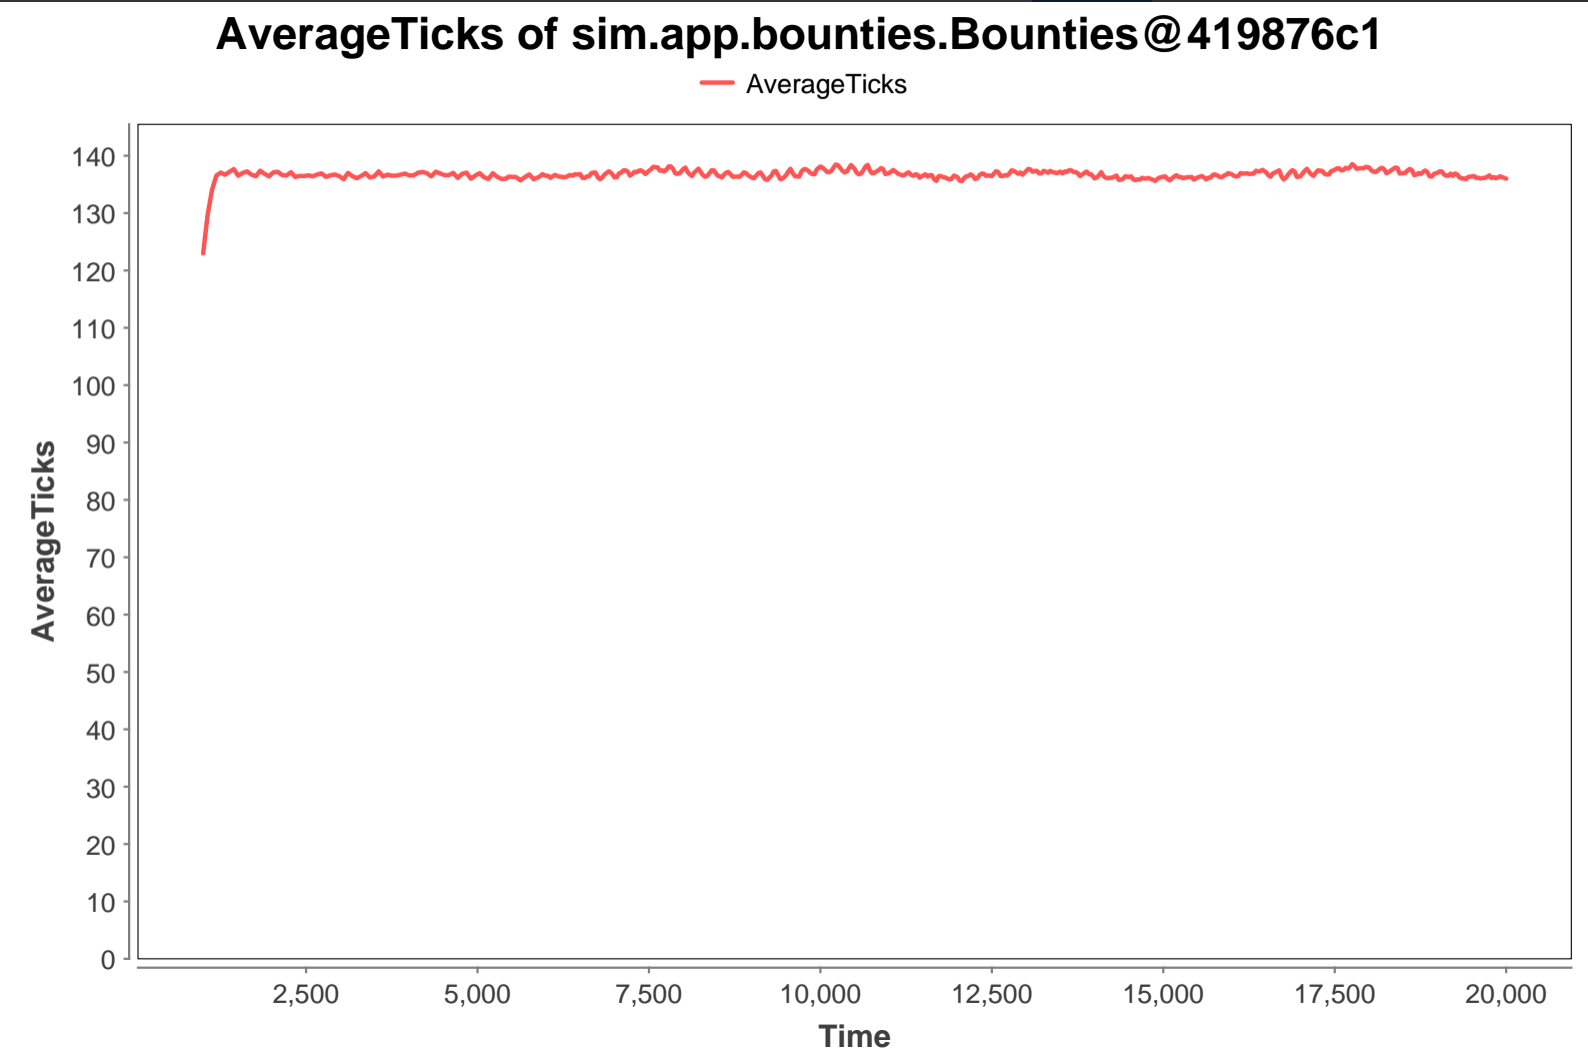
\includegraphics[width=8cm]{greedy2and10}
\caption{Jump-ship approach}
\end{figure}
% Qlearning
\begin{figure}[H]
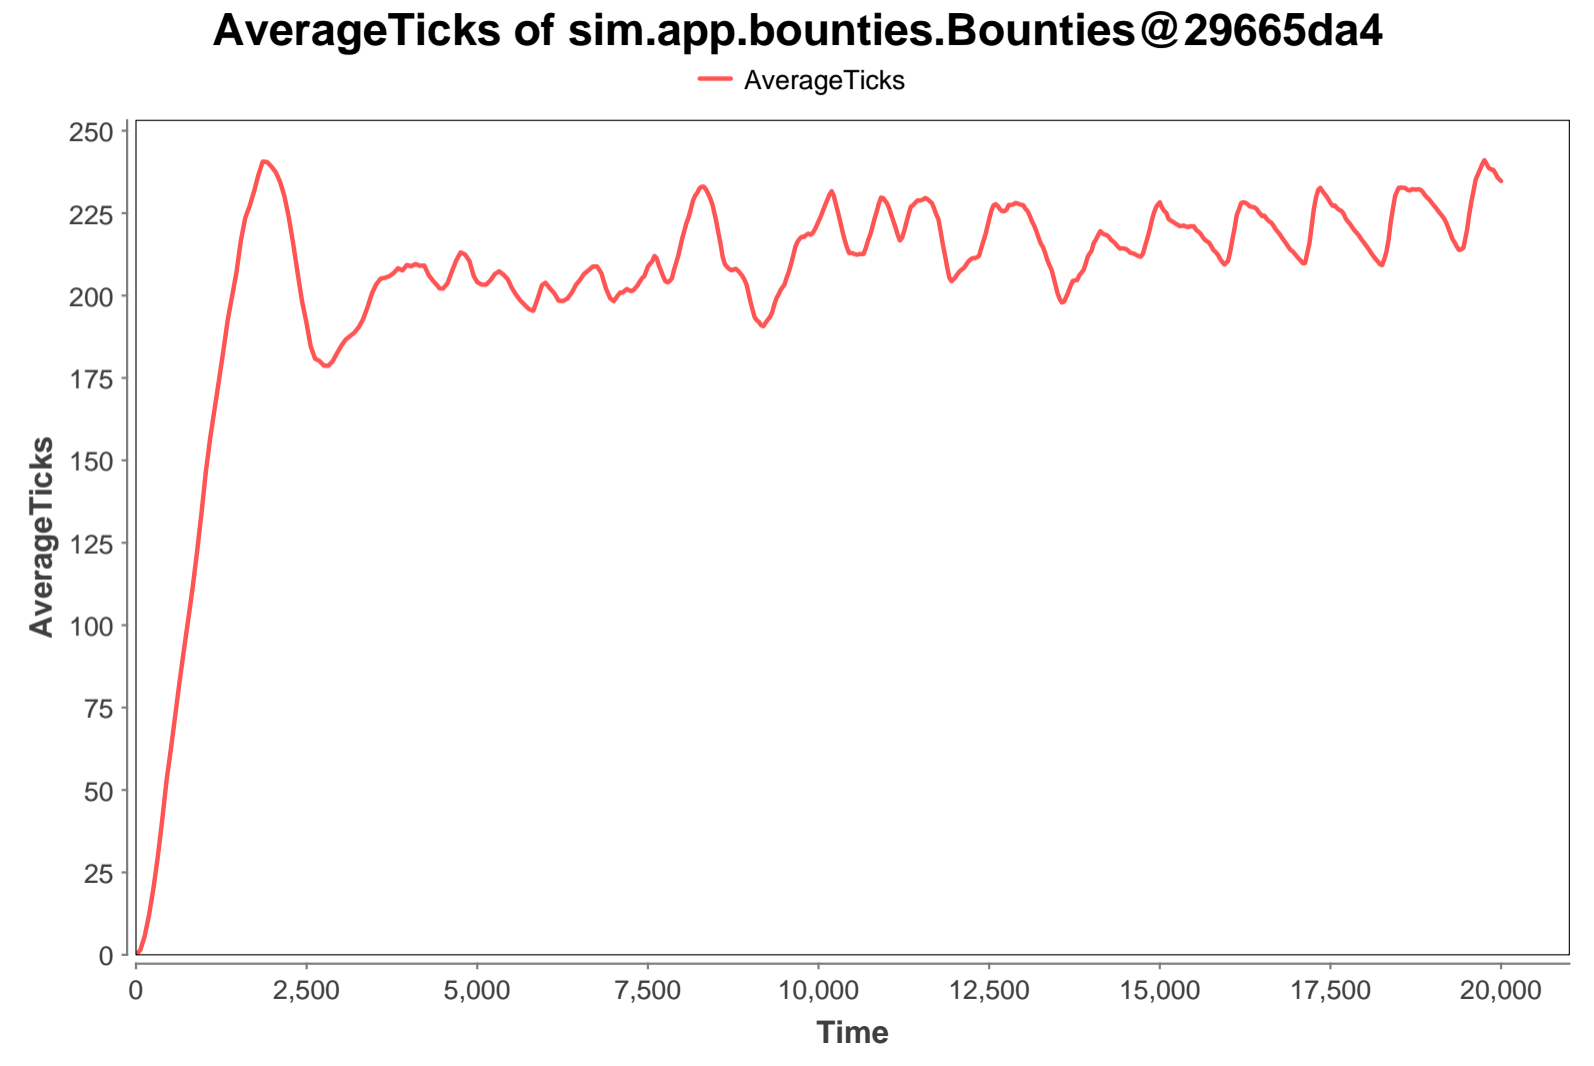
\includegraphics[width=8cm]{qlearning2and10}
\caption{Q-Learning approach}
\end{figure}
% DD
\begin{figure}[H]
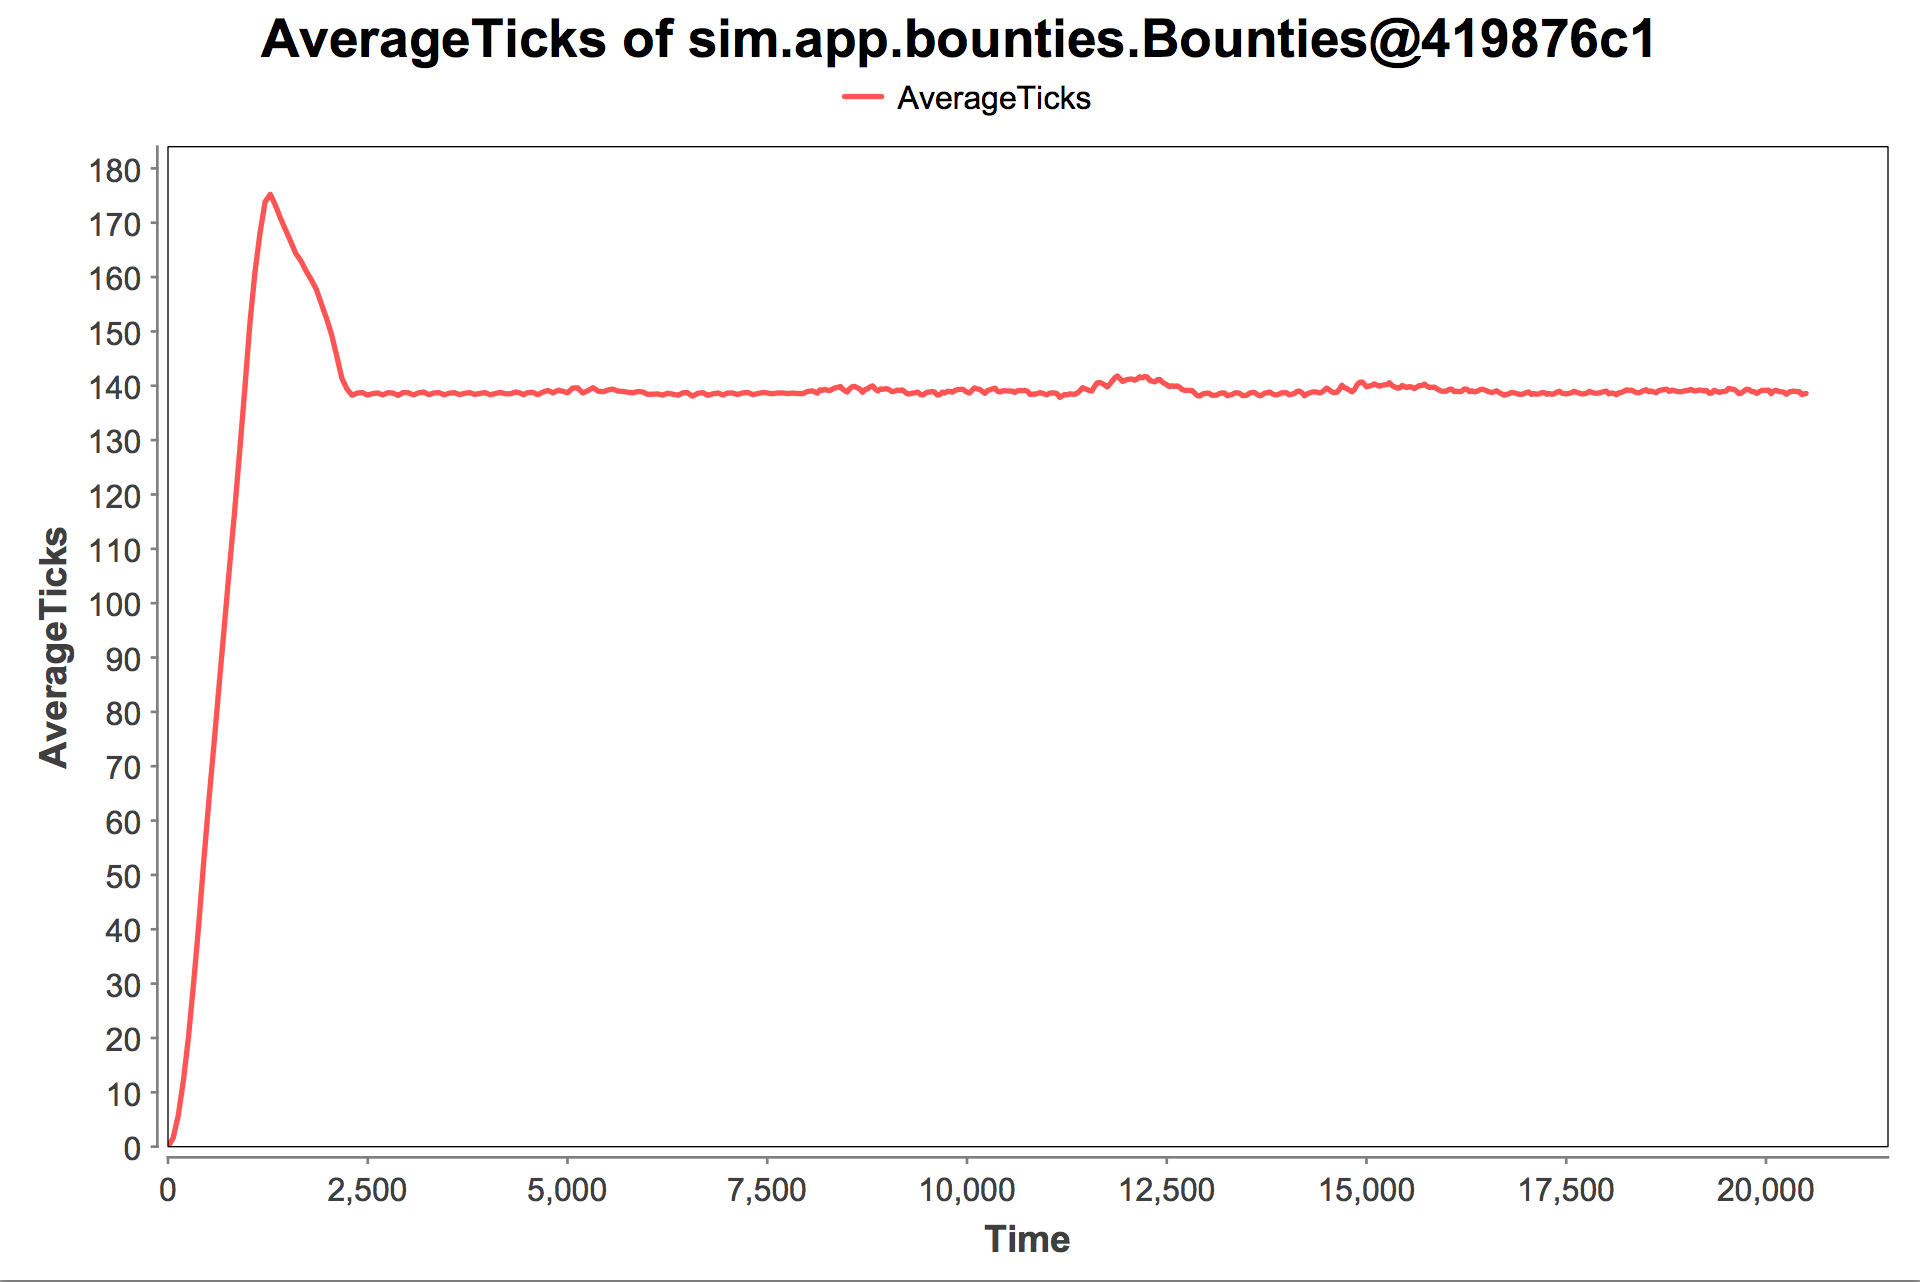
\includegraphics[width=8cm]{dd2and10}
\caption{DDLearning approach}
\end{figure}

\subsection{8 Robots 30 Tasks}
This experiment consisted of randomly placing 30 tasks, 1 goal location, and 8 robots on the field and then running the experiment for 20,000 time steps.

% Greedy
\begin{figure}[H]
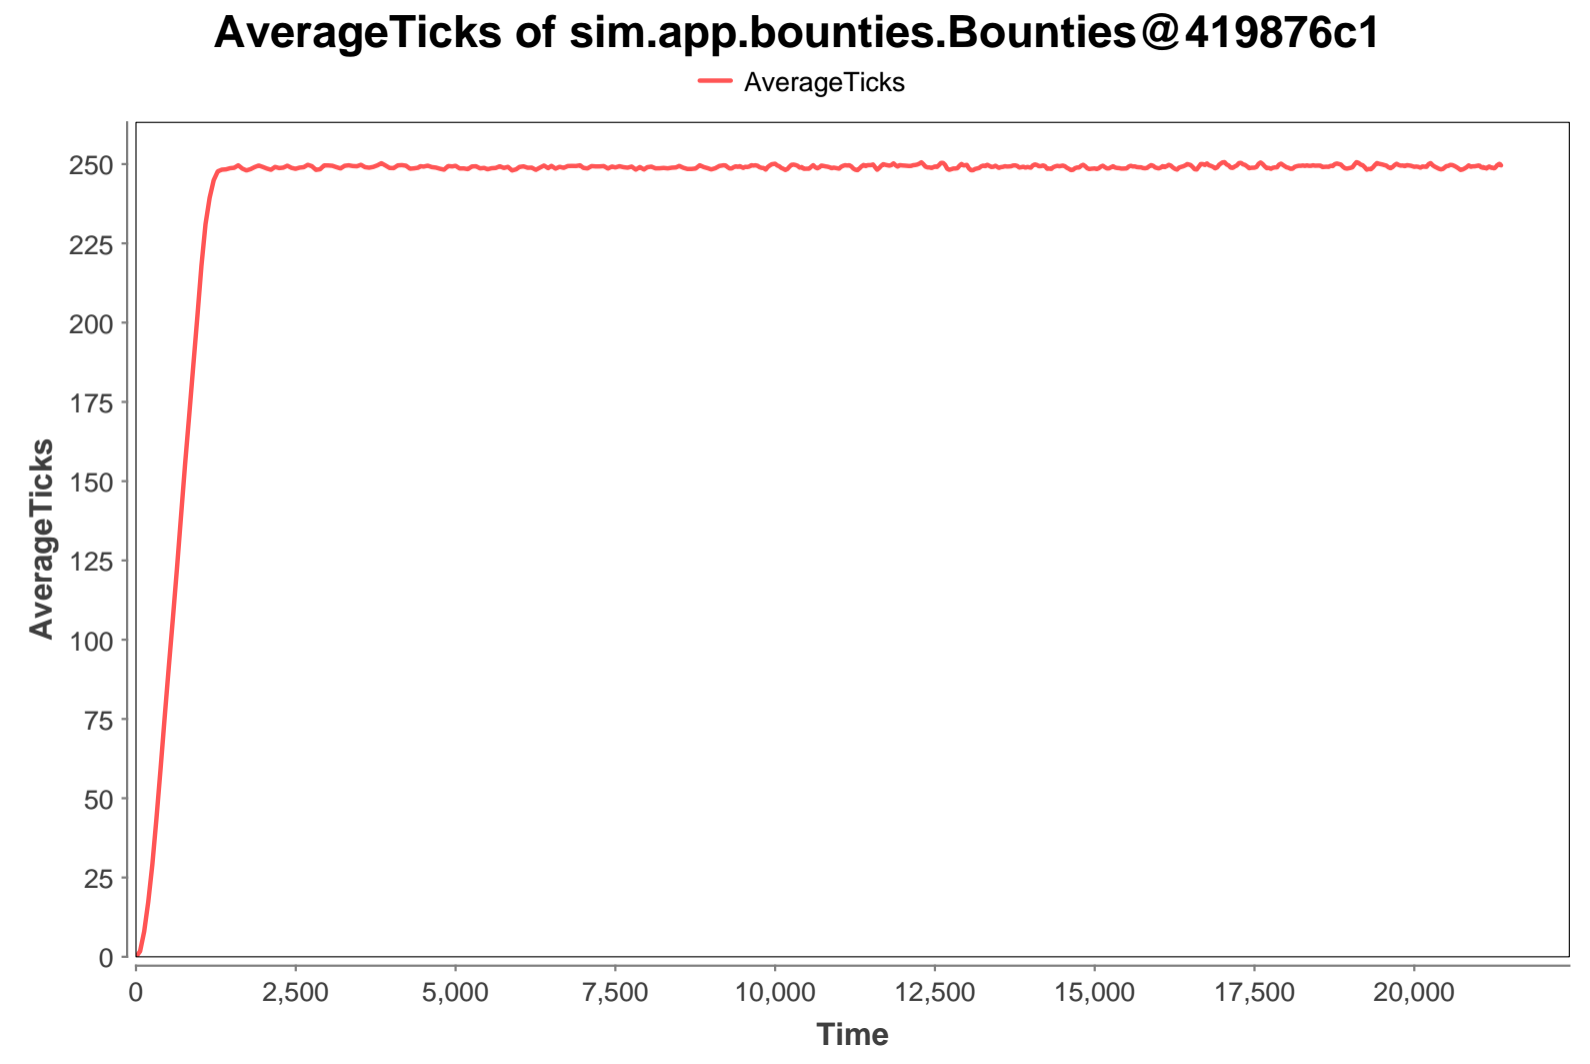
\includegraphics[width=8cm]{greedy8and30}
\caption{Jump-ship approach}
\end{figure}
% Qlearning
\begin{figure}[H]
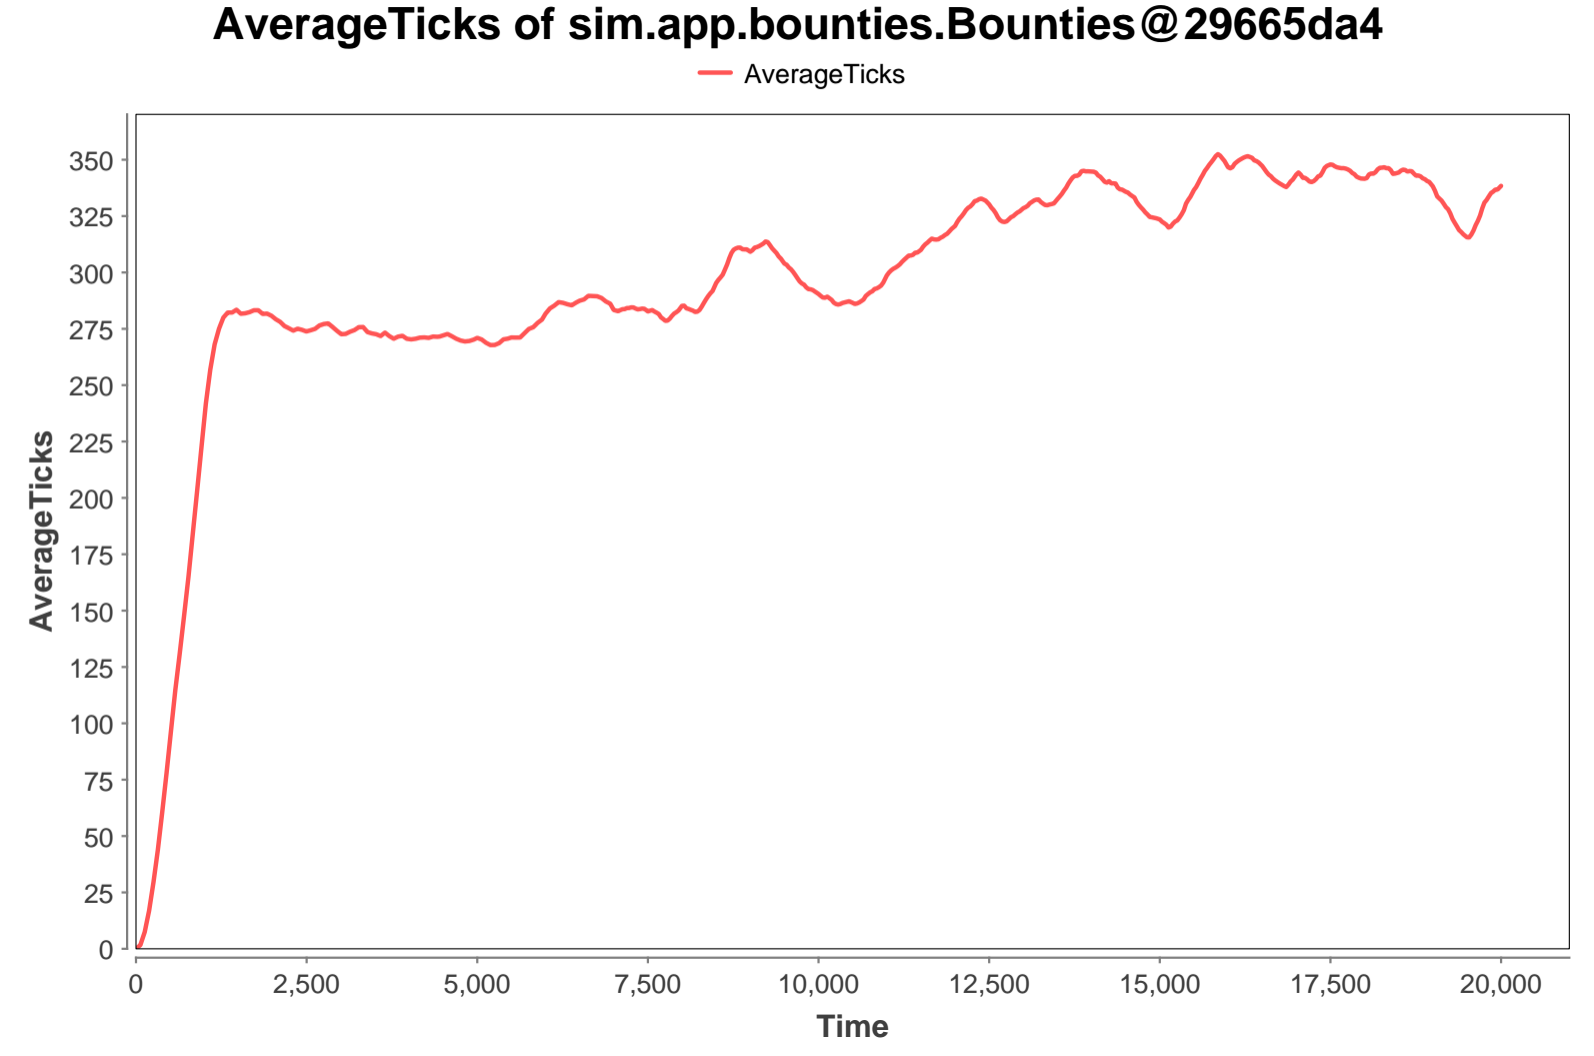
\includegraphics[width=8cm]{qlearning8and30}
\caption{Q-Learning approach}
\end{figure}
% DD
\begin{figure}[H]
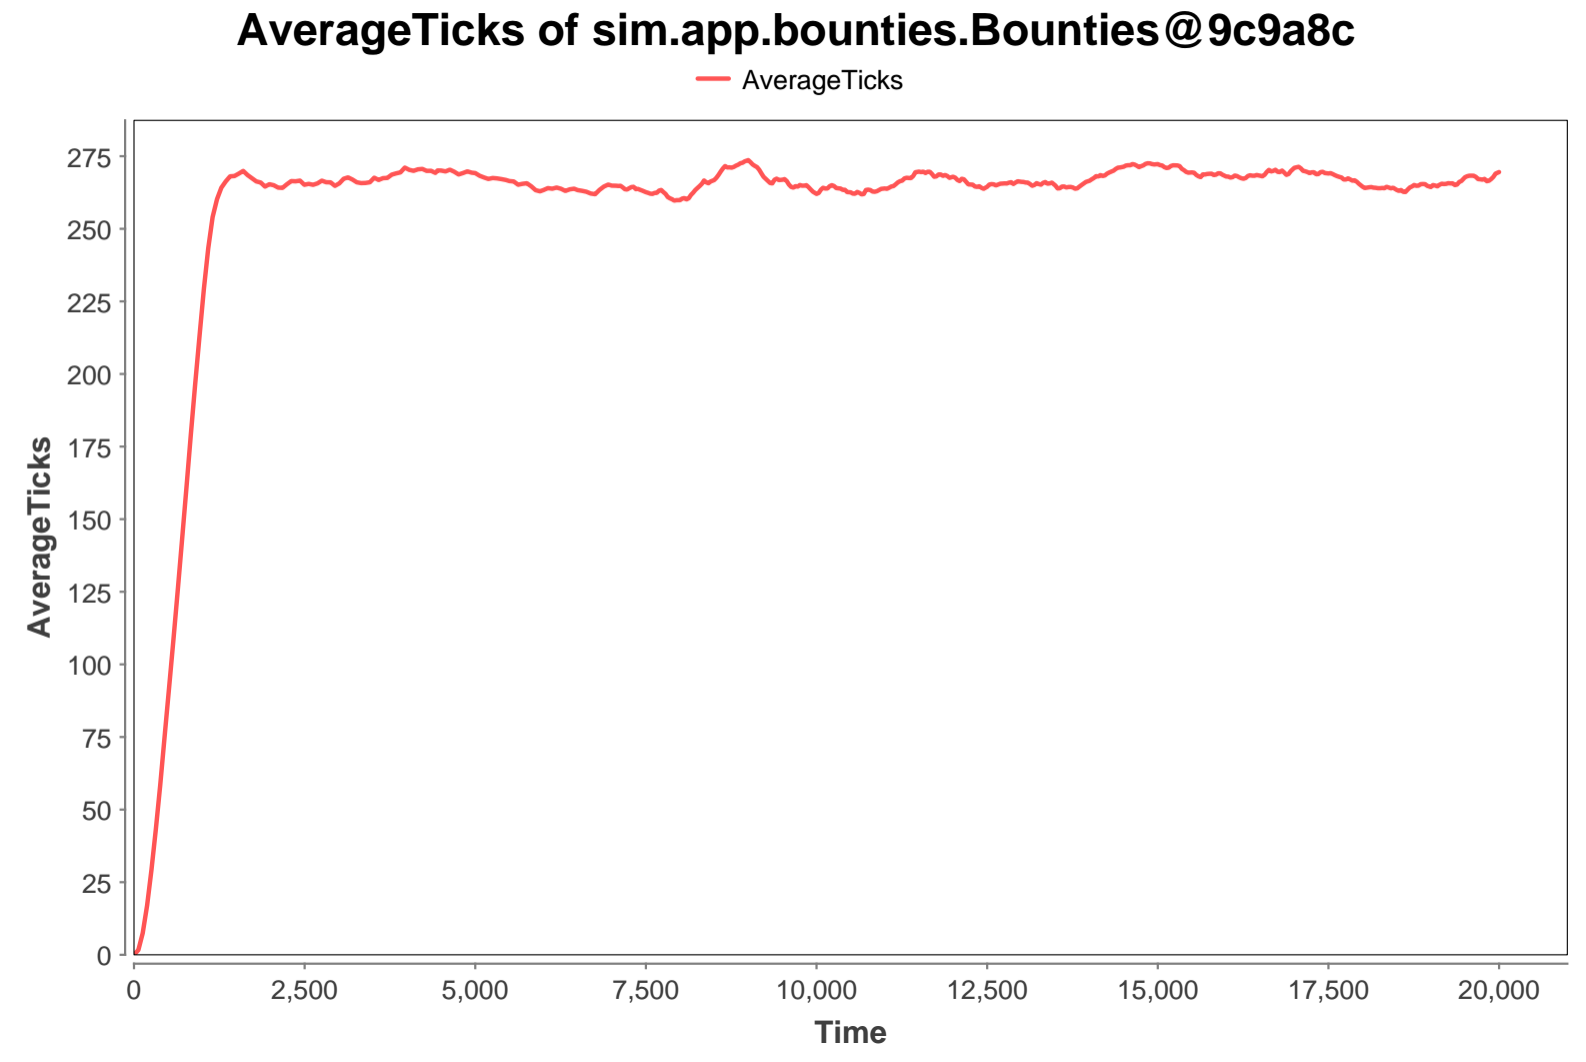
\includegraphics[width=8cm]{dd8and30}
\caption{DDLearning approach}
\end{figure}

\subsection{8 Robots 300 Tasks}
This experiment consisted of randomly placing 300 tasks, 1 goal location, and 8 robots on the field and then running the experiment for 20,000 time steps.  Due to the excessive computation time greedy approach was not used.

% Qlearning
\begin{figure}[H]
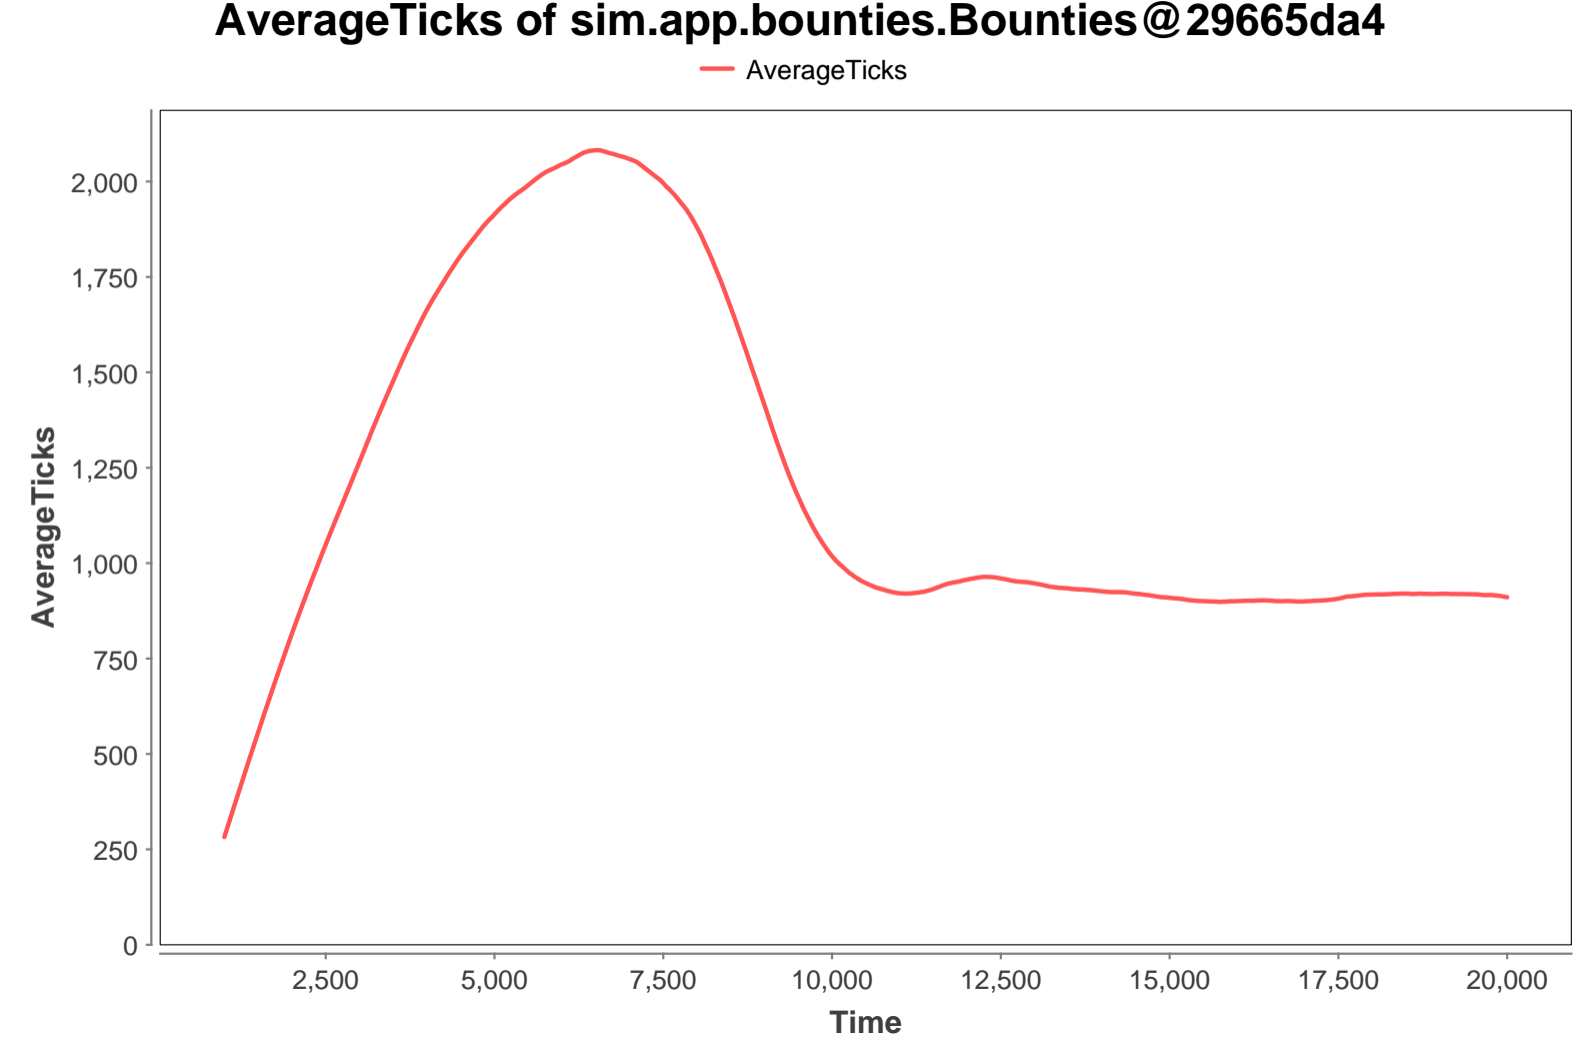
\includegraphics[width=8cm]{qlearning8and300}
\caption{Q-Learning approach}
\end{figure}
% DD
\begin{figure}[H]
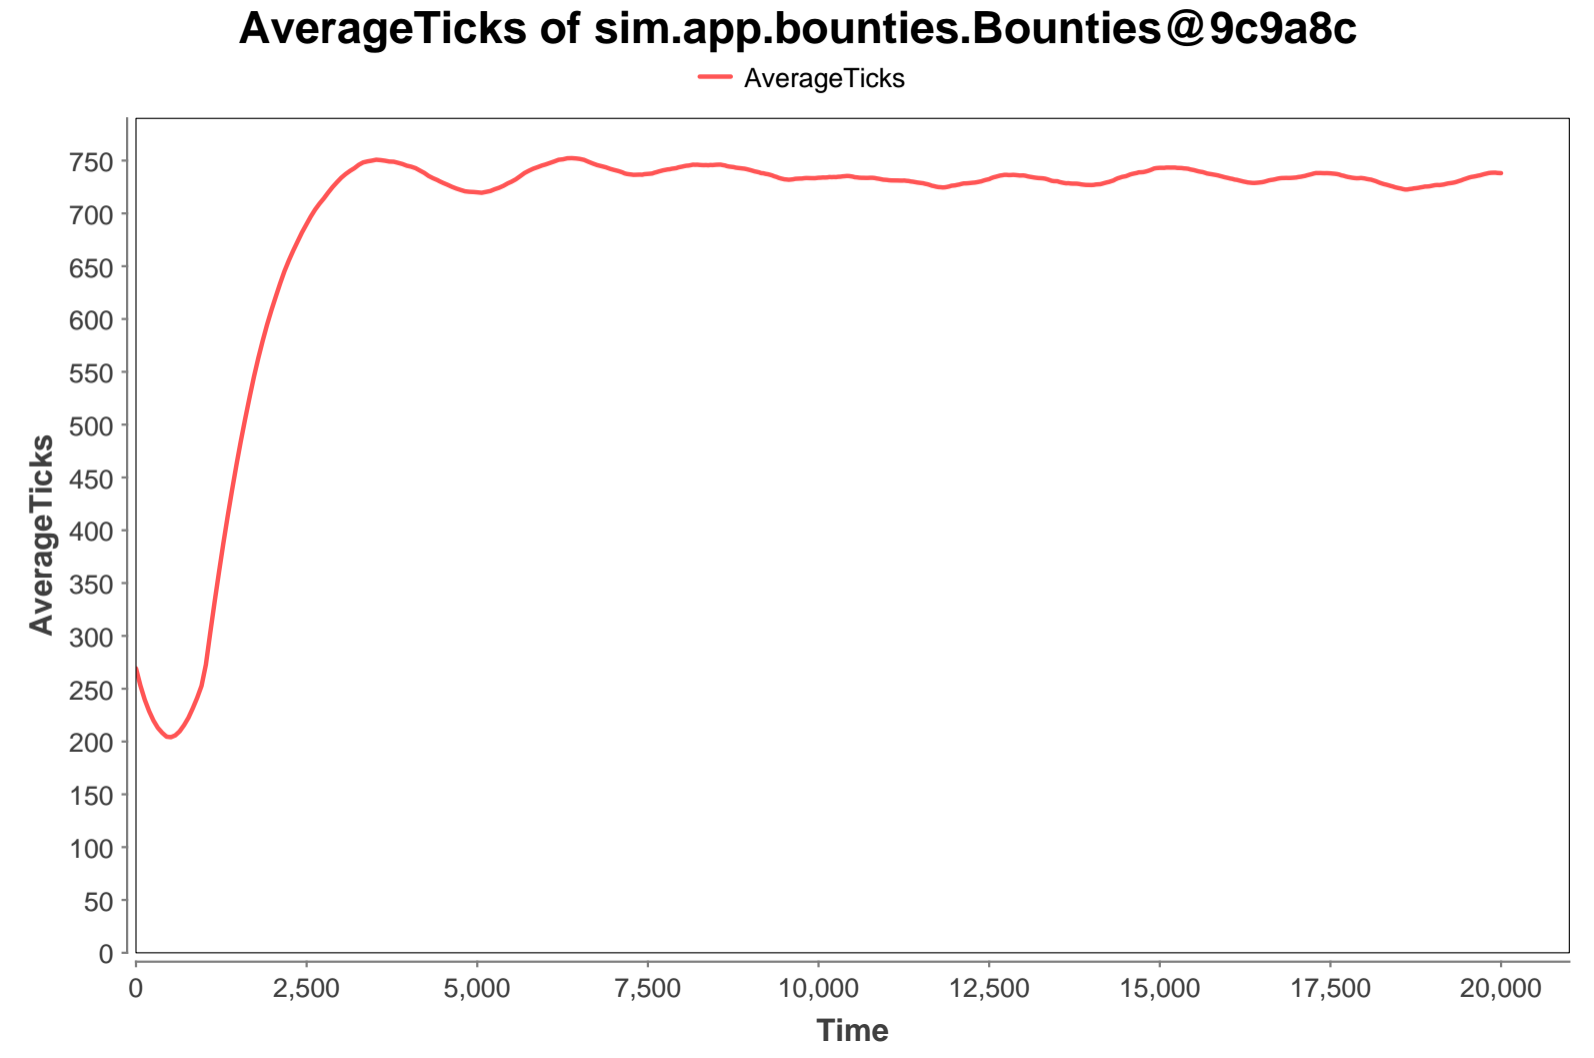
\includegraphics[width=8cm]{dd8and300}
\caption{DDLearning approach}
\end{figure}

\subsection{2 Robots 10 Tasks Configured}

This experiment consisted of configuring the locations of 10 tasks and randomly placing 1 goal location, and 2 robots on the field and then running the experiment for 20,000 time steps.  The tasks were configured in order to accentuate the bounty mechanism by placing half of the tasks far away from the goal and the other half around the goal.  This is similar to the \textit{forager-protector} scenario described in \cite{Campbell2010}, except with ours the distance implies the type of task.  Where there are two types of tasks one to protect the goal (close) and the other to go forage (far from goal).
\begin{figure}[H]
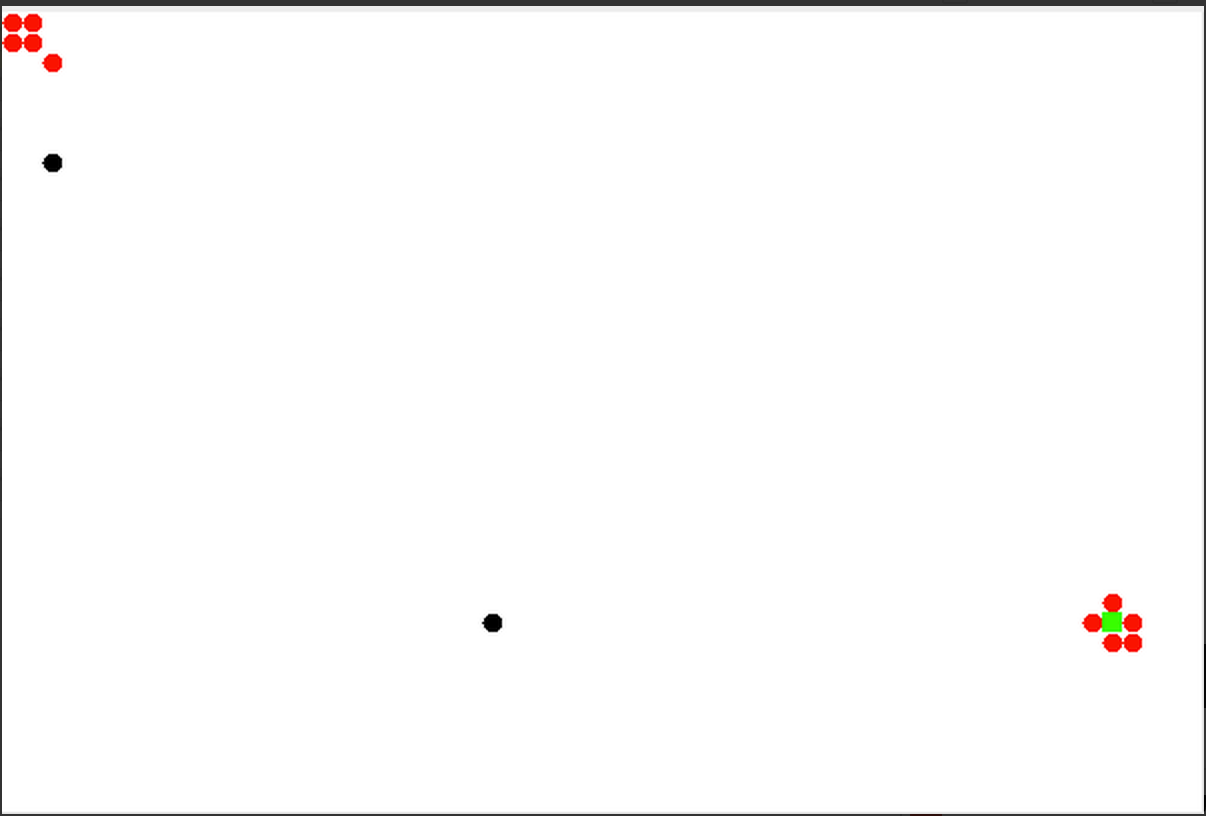
\includegraphics[width=8cm]{specialConfig}
\caption{Configuration of field.  Red = task, Green = goal, Black = Robot}
\end{figure}
% Greedy
\begin{figure}[H]
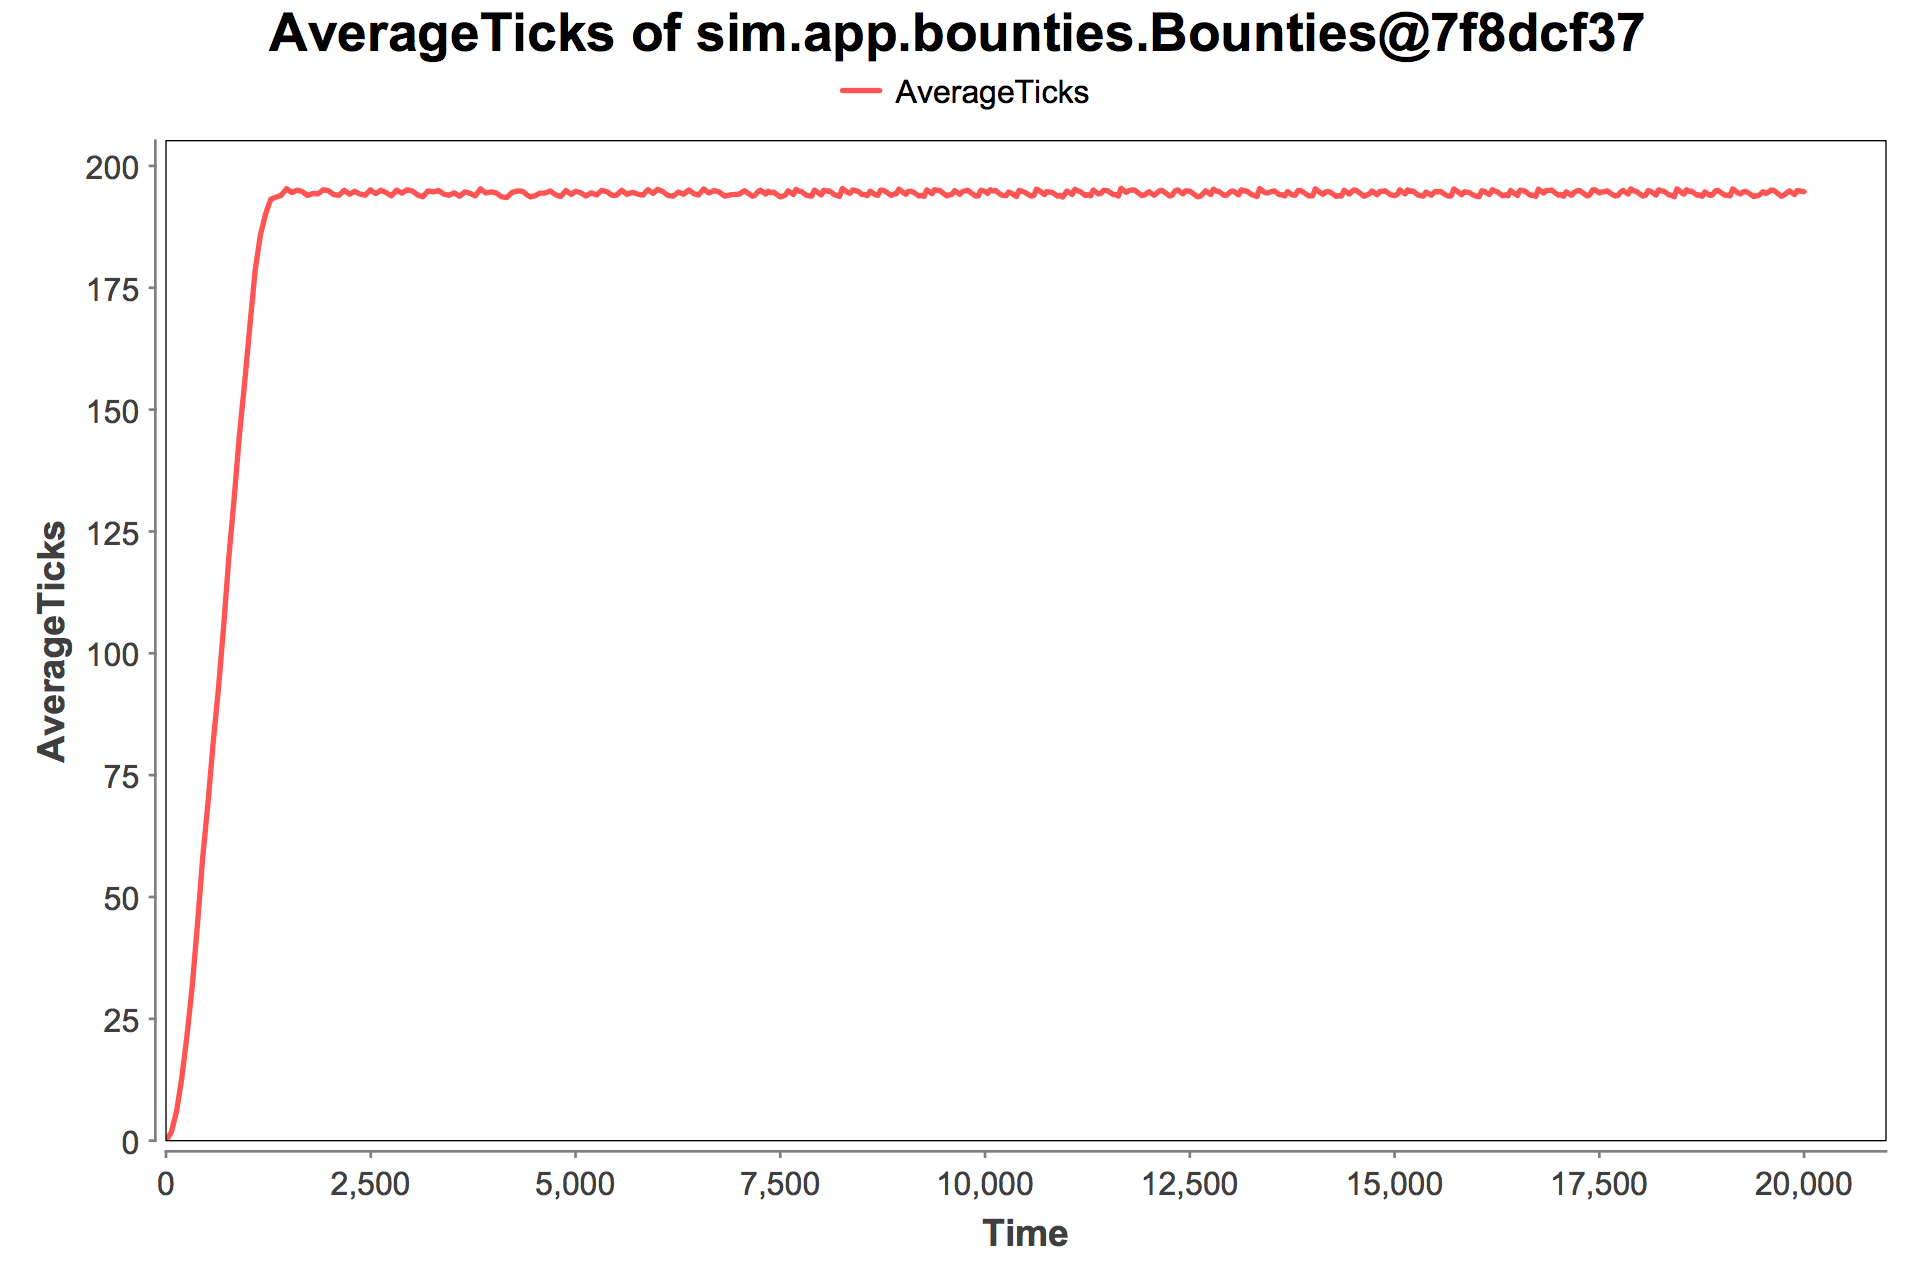
\includegraphics[width=8cm]{specialgreedy2and10}
\caption{Jump-ship approach}
\end{figure}
% Qlearning
\begin{figure}[H]
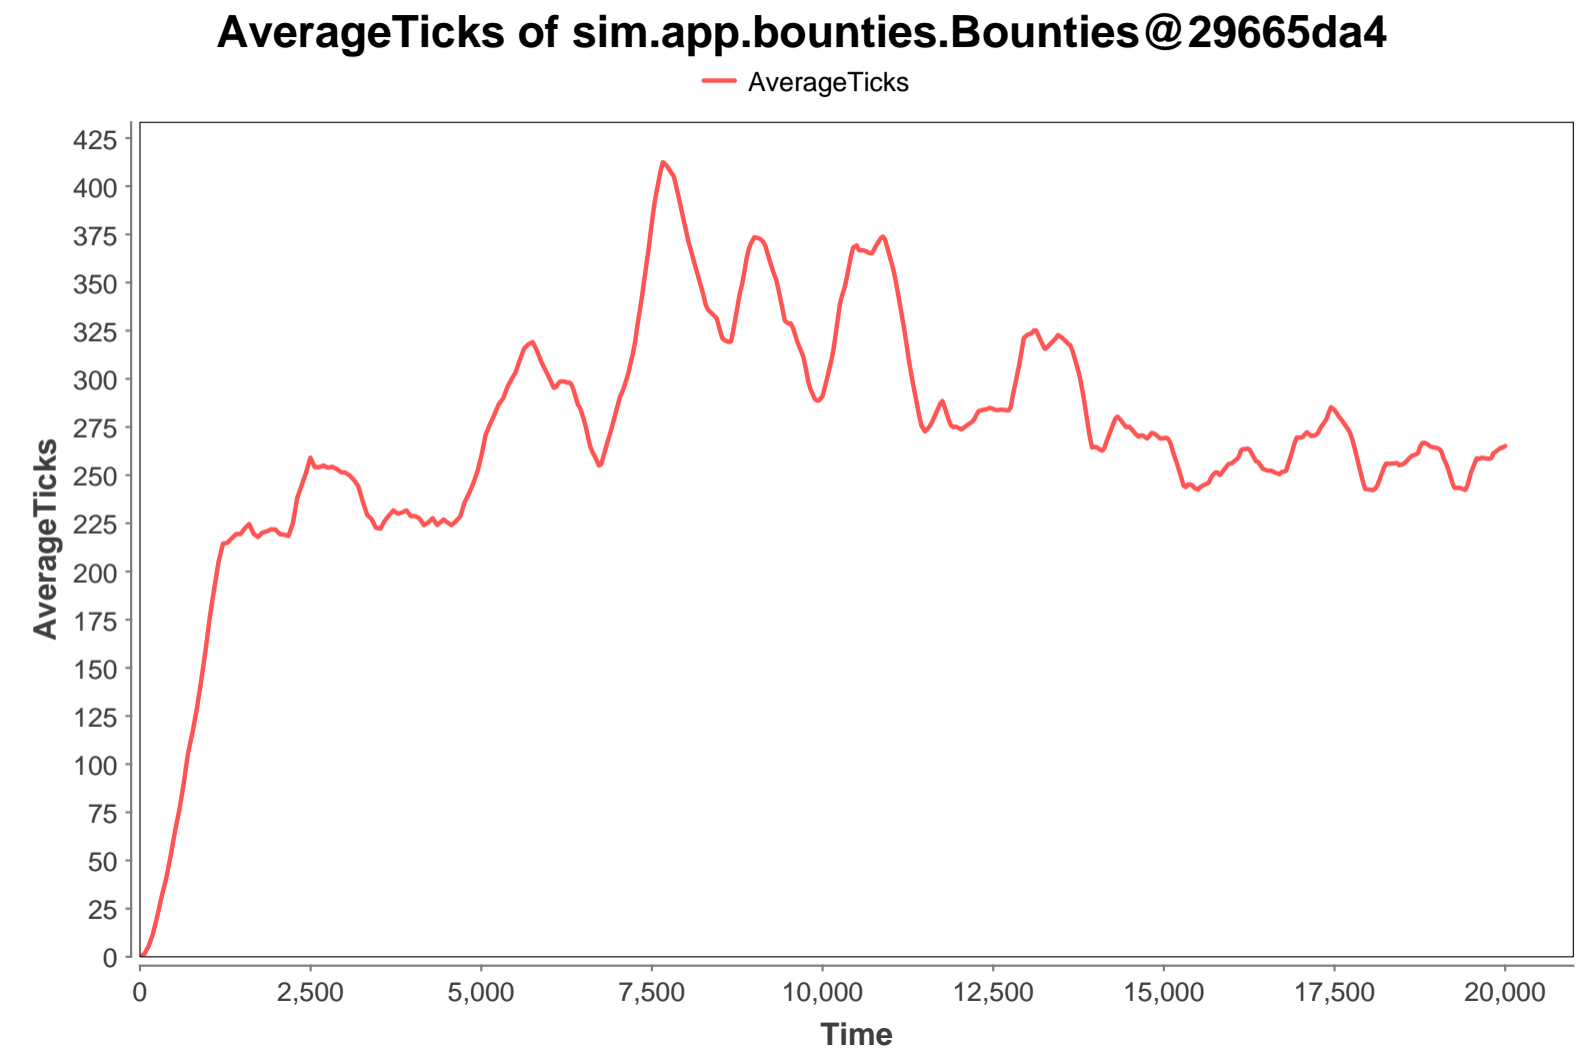
\includegraphics[width=8cm]{specialqlearning2and10}
\caption{Q-Learning approach}
\end{figure}
% DD
\begin{figure}[H]
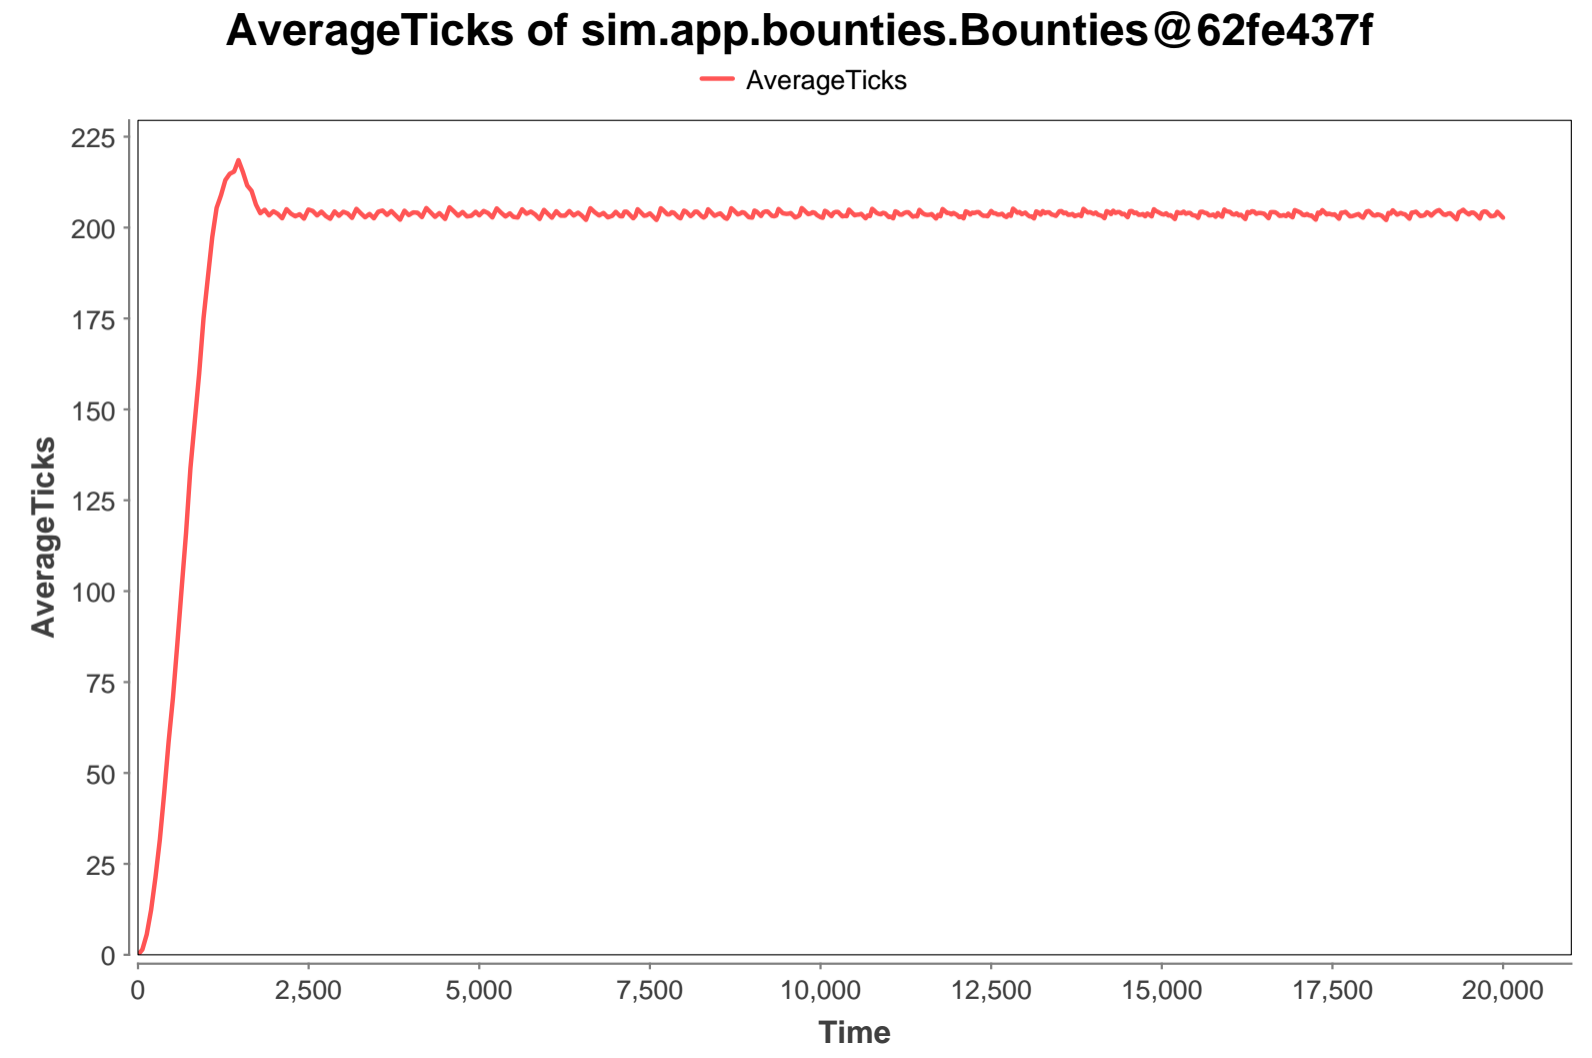
\includegraphics[width=8cm]{specialdd2and10}
\caption{DDLearning approach}
\end{figure}


\section{Analysis and Discussion}

As the graphs show in each experiment the Jump-ship approach (the greedy approach) outperforms both DDLearner and the Q-Learning algorithms.  This is mainly because this algorithm has full knowledge of what everyone is doing and their measure of how good they are going to be at it every time step.  This approach is not a viable option to use when the number of tasks or number of robots increases as the communication overhead is too great.  As is seen in the case with 8 robots and 300 tasks the Jump-ship approach was not able to perform in a reasonable amount of time compared to the DDLearner or the Q-Learner.

The Q-Learning approach based off of our limited experiments did not converge (except for the 300 task case where it did not perform as well as the DDLearner) and did not appear to be improving as time increased past 20,000 time steps.  This may be due to both the size of the q-table and the non-stationary environment.  In contrast, the DDLearner was able to converge and did relatively similar to the Jump-ship approach.  One benefit of the DDLearner approach is that it does not require the full information that the Jump-ship algorithm requires.  The only thing is that the space required grows linearly with the number of tasks.

% Want to do this in the future...We analyzed both convergence and fairness to the tasks as measured by average time the tasks were on the field.

\section{Robot Demonstration}
We also demonstrated the system on two Darwin-OP humanoid robots.  We placed a Robocup regulation size ball midway between center and the goal on both sides of the field.  The robots were tasked to go to the ball and kick the ball into the goal and then to go to the center of the field.  The robots were not told which task they should be responsible for, the goal of the experiment was to show that the robots could learn their role in the simulation and then transfer that behavior to the robots.    

We ran the simulation for 5000 time steps until the DDLearner robots converged to a set of roles where one robot took one task and the the other took the other task.  Then we switched the controller mechanism to move the Darwin-OPs and update the simulation with their location data.  The robots were able to successfully complete their separate tasks using the learned behaviors from the simulation.  A video of the demonstration can be found \url{http://youtu.be/LXiHaUqBWLI}.

\section{Future Work}
The future work will be focused on tasks that require multiple robots and therefore cooperation within a competitive environment.  We intend to carry out experiments in this ST-MR-IA environment to explore how the DDLearner and bounties work. This needs to be done because this type of problem is NP-Hard and will show how well bounties actually do.  We would study the emergent coalitions from just our DDLearner and compare it to a Coalition learning algorithm.  We would like to analyze both convergence and fairness to the tasks as measured by average time the tasks are on the field.

\bibliographystyle{ecai2014}
\bibliography{cs880}
\end{document}
